\chapter{Research Context}
\graphicspath{{Chapter2/Figs/}{Chapter2/Figs/}}

This chapter describes the research question's context and the current literature findings. The reader is educated on neuroscientific limitations, the state of current non-invasive BCIs, the motivation for developing cloud-based and mass-market-ready BCI software and the general definition of a N/CI.

\section{Limitations of BCIs}
\label{chapter2-limitations-of-bcis}

The possibilities of BCIs are not without limitations. In addition to the hardware limitations, the author addresses a broader issue related to neuropsychology that directly correlates with the software aspects, in addition to the challenges of computability.

\subsection{Decoding brain data}
\label{chapter2-decoding-brain-data}

It is important to emphasise that the task of decoding neural data is different from decoding thoughts, which is a critical factor for software. Moreover, decoding neural data and extracting the thoughts behind it so that the software can understand them are disciplines on their own. For example, getting computers to recognise letters written on a photograph is a very different problem from reading the written words in the sentences (i.e. computer vision and natural language processing). Another part is understanding the sentences and their meaning, as in natural language understanding (NLU).

NLU is considered an AI-hard problem, which means that the difficulty of these computational problems is assumed to be equivalent to solving the central problem of artificial general intelligence\footnote{Based on the assumption that general human-level intelligence could be computable.} \citep{demasi_theoretical_2010}. Understanding less structured data, such as neural data, is more complicated than understanding structured and human-generated syntax such as written language because it contains more hidden features and semantics than a paragraph of text. As a result, the author strongly assumes that understanding neural data can also be considered an AI-hard problem.

\subsection{Abstract thoughts}
\label{chapter2-abstract-thoughts}

To further emphasise the complexity of interpreting neural data, a practical example will be presented: Imagine a red house in the middle of a forest. Depending on the individual thought process, one might imagine the house with temporary visual imagery in mind, as in visual thinking, or one might imagine it more verbally, such as conceptually comprehending each word sequentially of what a red house is and that it is located in a forest \citep{amit_asymmetrical_2017} as shown on \autoref{fig:visual-thinking}.

\begin{figure}[ht]
  \centering
  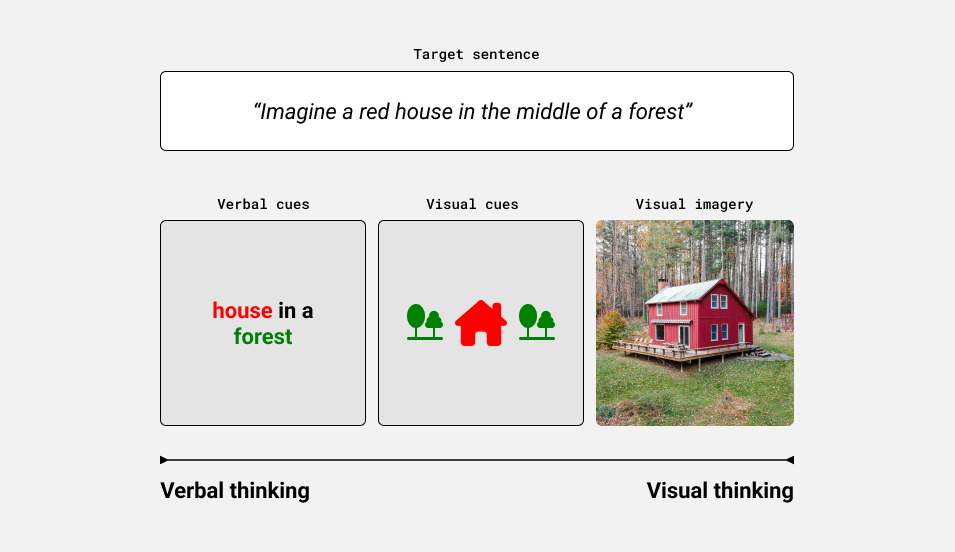
\includegraphics[width=\linewidth]{visual-thinking.png}
  \caption{Difference between verbal and visual thinking using the target sentence of a red house in the middle of a forest}
  \label{fig:visual-thinking}
\end{figure}

Additionally, it should also be addressed that different types of thoughts exist at different levels of abstraction and complexity. One can assume that the visual image of a red house in the forest is more abstract and far-fetched than, say, the movement of one's own thumbs, which has a clear physical counterpart. It gets even more complicated when one imagines abstract concepts that are inconceivable to visualise, such as the idea of a company. A company is an abstract, collectively agreed upon concept without a clear physical counterpart\footnote{Some people might think of a company building when imaging a company, others might imagine their website, their logo or physical products.} and is, therefore, even less straightforward and more complex to decode the meaning of measured brain activity than the other mentioned examples of the red house.

\subsection{Technological limitations}
\label{chapter2-technological-limitations}

Most functional tasks of the brain are localised, which means that these signals are generated by local brain areas that can be identified, such as the motor cortex, which has been shown to be responsible for muscle movement as shown in \autoref{fig:fmri-scan}.

\begin{figure}[ht]
  \centering
  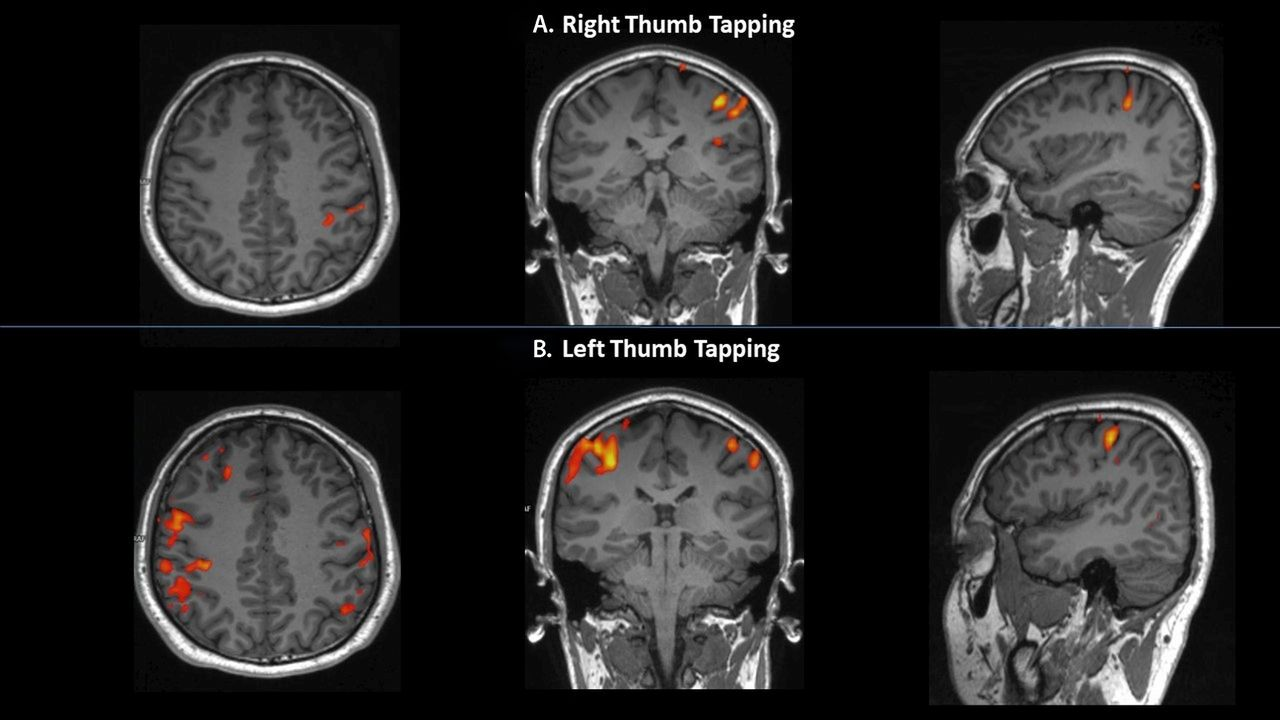
\includegraphics[width=\linewidth]{fmri-scan.jpg}
  \caption{Localised neurons during right and left thumb movement using functional magnetic resonance imaging (fMRI) \citep{rashid_bilateral_2018}}
  \label{fig:fmri-scan}
\end{figure}

Examining the areas of the brain responsible for activating individual muscle strands can yield a comparable response of muscle stimulation in the brain and thus be measured as input for BCI software to, e.g. move a prosthesis. However, the more specific, more behavioural and abstract the thoughts are, the less the brain areas are spatially visible. With the intention of identifying, e.g. the thought of a red house in a forest, the author has identified three technological limitations:

\begin{itemize}
  \item To understand single thoughts, it is essential to have sufficiently clear data with a certain level of detail (e.g., at the level of detail of eliciting action potentials of individual neurons\footnote{Action potentials are the fundamental neurobiological and neurochemical processes through which neurons transfer information to each other.}) and temporal precision (an action potential has a short duration of about one millisecond \citep{byrne_resting_2021}) to perform studies to extract possible localisation of individual thoughts. Current neuroimaging technologies cannot capture every process in sufficient detail of the entire brain at once to extract the activity of individual neurons while also having high temporal precision.
  \item Even if we could measure every single neuron in the brain with high temporal precision, we would have an extreme amount of data generated concisely. Let us say we would collect a float\footnote{The size of a float on a Windows 64-bit application is 4 bytes which was used for the calculation.} per neuron that represents the rate of change in voltage with respect to time with a frequency of 1 ms and then record each neuron in the brain a million times a second, taking into account that the average human brain has around 86 billion neurons; we would generate 305.53337637684 petabytes of data per second. This is currently not feasible for commercially available storage and processing resources.
  \item Even if we have the technology, it is a challenge because reproducibility of experiments is very difficult for neuroscientific studies (usually referenced as the replication crisis \citep{maxwell_is_2015}). It is probably impossible to generate clean-slate brain data that is comparable to previously recorded data since our neurophysiological brain tissue changes over time due to neuroplasticity \citep{puderbaugh_neuroplasticity_2022}, and since we are in different states of mind every millisecond of our existence, which can have different influences, such as insufficient sleep, something disturbing someone, mental distraction due to an important event that may have occurred since the last measurement, or a salient thought that randomly occurs.
\end{itemize}

\subsection{Lack of data}
\label{chapter2-lack-of-data}

As pointed out in the previous section, the last two points depend on advances in storage systems or the possibility that we do not actually need such precise brain data to understand single thoughts. However, to address the first point, some promising solutions already exist for measuring large parts of the brain with high temporal and spatial precision, such as time-domain functional near-infrared spectroscopy (TD-fNIRS), which the company Kernel employs in its Flow device \citep{ban_kernel_2021}. The TD-fNIRS system detects changes in concentrations of oxygenated and deoxygenated brain cell activity by using near-infrared light in response to neuronal activity. According to Kernel, the precision of TD-fNIRS is sufficient for better understanding the brain and using it for BCI applications. They, however, claim that collecting and organising longitudinal brain data from a variety of subjects is the key to solving the most difficult challenges in neuroscience \citep{kernel_hello-humanitypdf_nodate}.

\newpage

Based on Kernel's claim, a recent publication from 2022 also claims that even data sets with several hundred people are too tiny to offer insights about the brain consistently; as a result, most published neuroscience studies with dozens or even hundreds of people could all be incorrect \citep{marek_reproducible_2022}. In such research, brain tissue and activity variations have been linked to variances in cognitive capacity, mental health, and other behavioural features. In addition, it has been shown in numerous studies that understanding the brain in more depth may help to distinguish people with depression. Neuromarkers\footnote{A neuromarker is a biomarker that is based on neuroscientific data to detect biological properties such as, e.g. a disease or illness \citep{jollans_neuromarkers_2018}.} of behavioural features are frequently sought in studies. The recent publication from \citeauthor{marek_reproducible_2022} claims that most of these so-called neuromarkers would not work when the collected data set is more extensive, which would pose a general problem for the field of neuroscience. UK Biobank's collection of brain scans is one of the first efforts to solve this problem \citep{noauthor_imaging_nodate}, but it is still far from what we might need since, e.g. Marek himself claims that we might even need millions of data sets to start understanding the brain \citep{callaway_can_2022}. This is both fascinating and a possible significant constraint for BCIs, because understanding the brain is essential to making sense of the measured data to interface with it.

However, there is the other side of this argument from people like Andrew Ng, artificial intelligence pioneer and founder of the Google Brain research lab. He believes that machine learning, which underpins all BCI software, should be developed in a data-centric manner, which means that the quality of the data on which models are trained should be as high as possible to answer specific research questions \citep{brown_why_2022}. However, this brings us back to the replication crisis, which is the difficulty in generating clean brain data comparable to previously collected data due to the nature of our ever-changing consciousness. 

Ultimately, there will almost certainly always be a mix of both approaches. As a result, for production- and mass-market-ready BCIs, a relatively large amount of qualitative brain data collected in specific and reproducible experiments or environments is required. This is where high-end, customer-focused BCIs could come into play because the adoption rate of a device suitable for everyday use is higher than the number of subjects in research labs, resulting in larger and more longitudinal datasets. This, combined with more targeted experiments, improved neuroimaging technologies, and advances in machine learning, could unlock enormous potential in brain research.

\section{BCI landscape}
\label{chapter2-research-landscape}

This section will discuss the current state of non-clinical and non-invasive BCIs, their applications and the distinctions within their software offerings.

\subsection{Real-world BCI applications}
\label{chapter2-real-world-bci-applications}

As mentioned in \autoref{chapter1-background}, consumer-oriented BCI products are already commercially available. OpenBCI, a non-medical BCI company, does not provide a specific use case but hardware, as depicted on \autoref{fig:openbci}, and software which is universally applicable. It can be used in research where EEG is used or in developing BCI applications. Several neurofeedback or research apps have been created using OpenBCI's products \citep{openbci_openbci_nodate}. Taking this information into consideration, we can see that the OpenBCI customer is responsible for developing their own BCI application or incorporating it into their research, rather than having a sophisticated end-user application from OpenBCI.

\begin{figure}[!ht]
  \minipage{0.32\textwidth}
  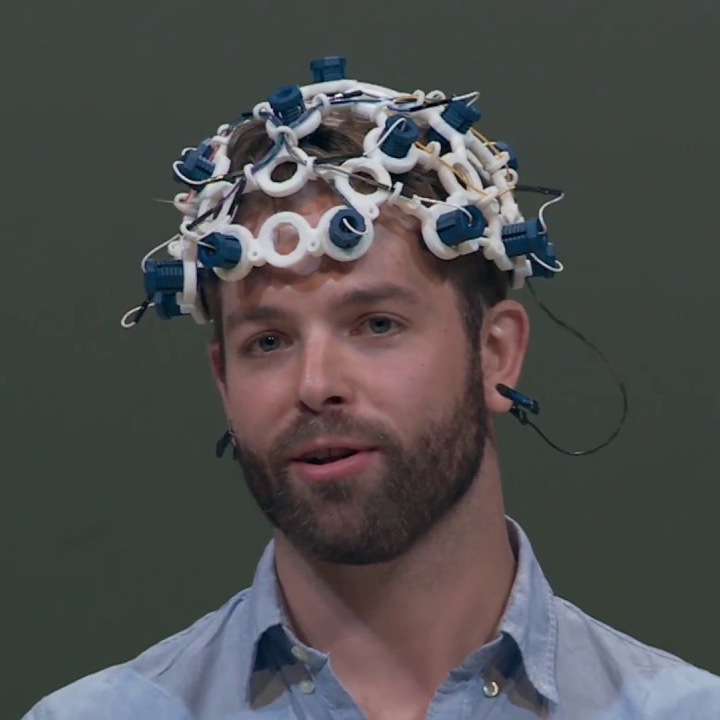
\includegraphics[width=\linewidth]{openbci.jpeg}
  \caption{OpenBCI's EEG \\ device \citep{be_superhvman_conor_2017}}
  \label{fig:openbci}
  \endminipage\hfill
  \minipage{0.32\textwidth}
  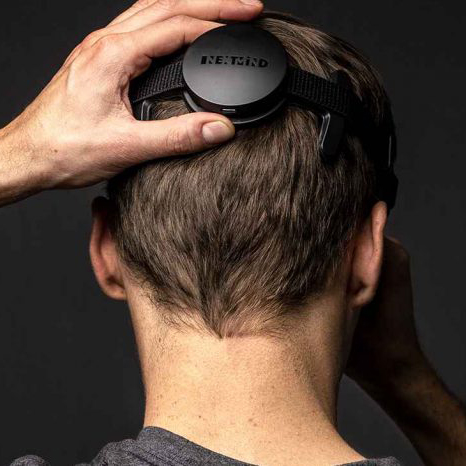
\includegraphics[width=\linewidth]{nextmind.jpeg}
  \caption{NextMind's BCI \\ device \citep{louise_neurotechnology_2019}}
  \label{fig:nextmind}
  \endminipage\hfill
  \minipage{0.32\textwidth}%
  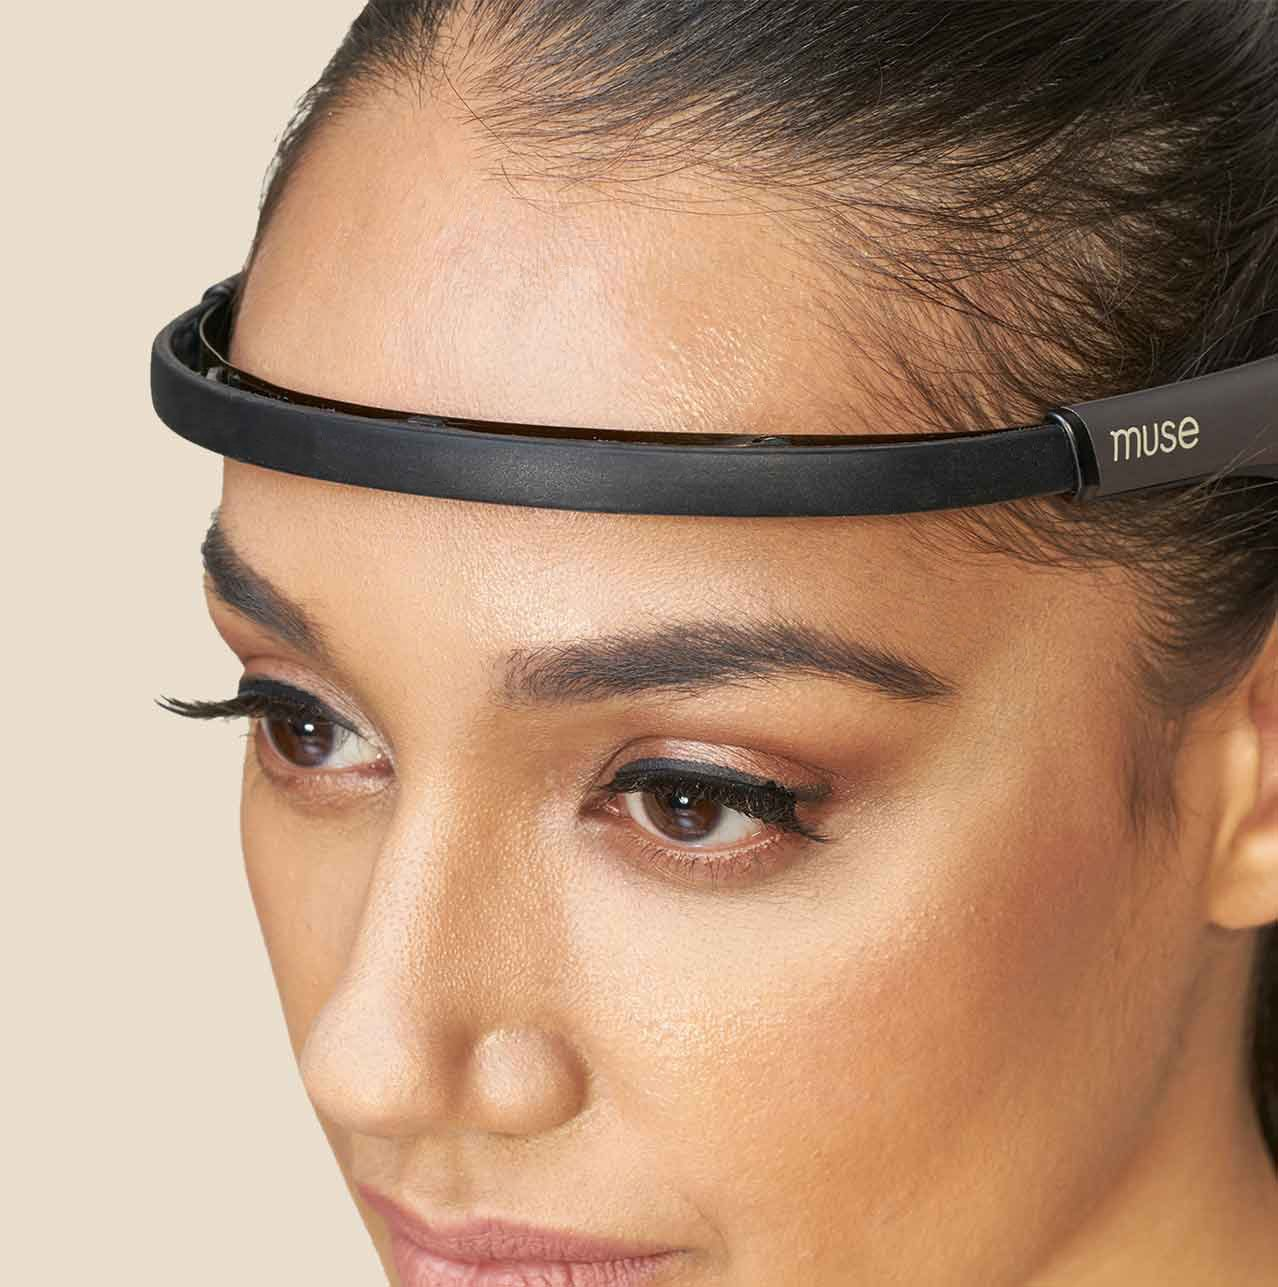
\includegraphics[width=\linewidth]{muse.jpeg}
  \caption{Muse's meditation \\ headband \citep{muse_muse_nodate}}
  \label{fig:muse}
  \endminipage
\end{figure}

Another example is NextMind's product, as shown on \autoref{fig:nextmind}. They do not focus on having an end-user application for their BCI, but they focus on offering an SDK for the Unity real-time engine to use their technology for brain-controlled actions in video games. One significant difference between NextMind and OpenBCI is that NextMind includes a built-in classification of brain waves captured by hardware, in this case, classification of active visual focus on virtual objects based on steady-state visual evoked potentials (SSVEP). Because their business model is presumably based on the unique selling point of their active visual focus classifier, NextMind does not provide access to the raw EEG data collected by the sensors. Nonetheless, NextMind's product is less focused on a specific use case, as its applicability is limited to games inside the Unity engine.

A relatively closed and specific BCI is, for example, the EEG headband by Muse as shown on \autoref{fig:muse}. Its purpose is to measure meditation and sleep. They also offer an end-user app to help people better understand their meditation and sleep and how to improve them. The Muse headband is not unidirectional BCI per se, as there is also biofeedback based on neural signals, but the vital difference between Muse and, e.g. OpenBCI is that they abstract away the neurotechnology. Users do not need to know anything about neuroscience, neurotechnology or the interpretation and classification of neural data to get useful functionality for their use case. They also do not need to understand the software system's underlying architecture. They only need to know how to pair the device with their smartphone via Bluetooth.

Aside from full-stack BCI solutions, where a company provides a complete BCI solution, including hardware and software, some companies focus solely on the software aspect. Neuromore, a company that provides a neural signal processing software platform, is one example. The company is hardware agnostic, which means one can plug any hardware or sensor into their computer and connect it to the Neuromore Studio software.

\begin{figure}[ht]
  \centering
  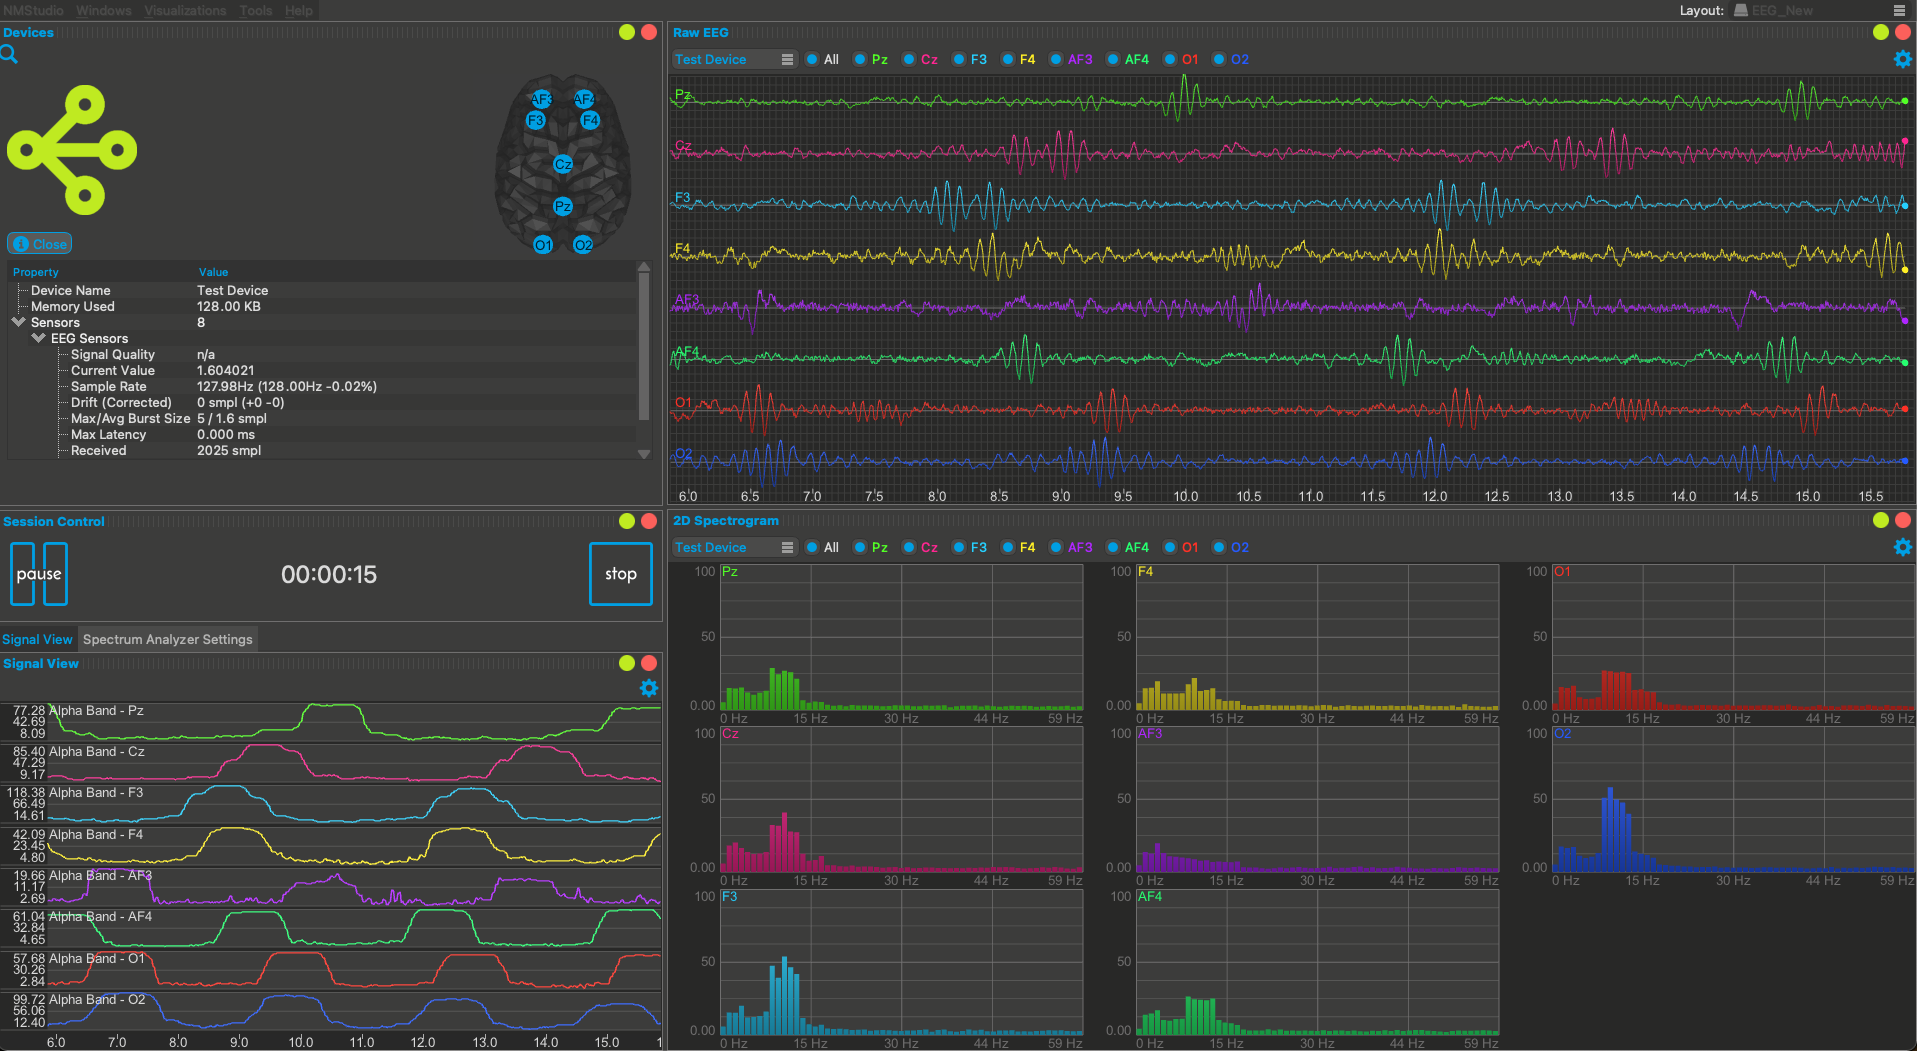
\includegraphics[width=\linewidth]{neuromore.png}
  \caption{Screenshot of the Neuromore Studio software \citep{neuromore_neuromore_nodate}.}
  \label{fig:neuromore}
\end{figure}

Neuromore Studio, as shown on \autoref{fig:neuromore}, is free and open-source software that runs locally on various platforms. It provides a variety of drag-and-drop interfaces for creating and managing signal processing pipelines. For example, one can transform EEG data to extract band power, create triggers based on band power selection, and generate conditional outputs for a game to, e.g. move a character.

The author attempts to differentiate the offerings of the consumer-oriented BCIs mentioned: They either provide the hardware (with software that at least connects to the device) but are then more broadly applicable to use cases not defined by the company behind the BCI, such as OpenBCI, or they are application-specific in terms of both the software and the hardware, such as the Muse headband.

Although this thesis focuses on consumer-oriented BCIs, the applications of various BCI offerings can still be distinguished based on whether they are more consumer-oriented or research-oriented, such as the distinction between, e.g. NeuroSky, creating EEG-based BCIs for hobbyists and Emotiv's professional and expensive EEG systems, which are more research-oriented. However, NeuroSky and Emotiv provide a research version and a consumer or enterprise version of their software and hardware, aiming for general-purpose applicability across customer segments and use cases.

Other considerations include whether the applications are rather steady-state evoked, such as based on a frequency of noise laid on top of virtual objects to detect which object the person is looking at (e.g. as NextMind is doing), or whether they track the totality of mental states without evoking neural signals with external stimuli, such as in tracking sleep or concentration levels, both of which arise primarily evoked from inside the mind. This distinction can be made as passive, active or reactive BCI, as \citeauthor{alimardani_passive_2020} coined in their work on passive BCIs \citep{alimardani_passive_2020}. However, we do not want to include this dimension because it would introduce unnecessary and additional complexities related to the BCI software application layer.

\begin{figure}[ht]
  \centering
  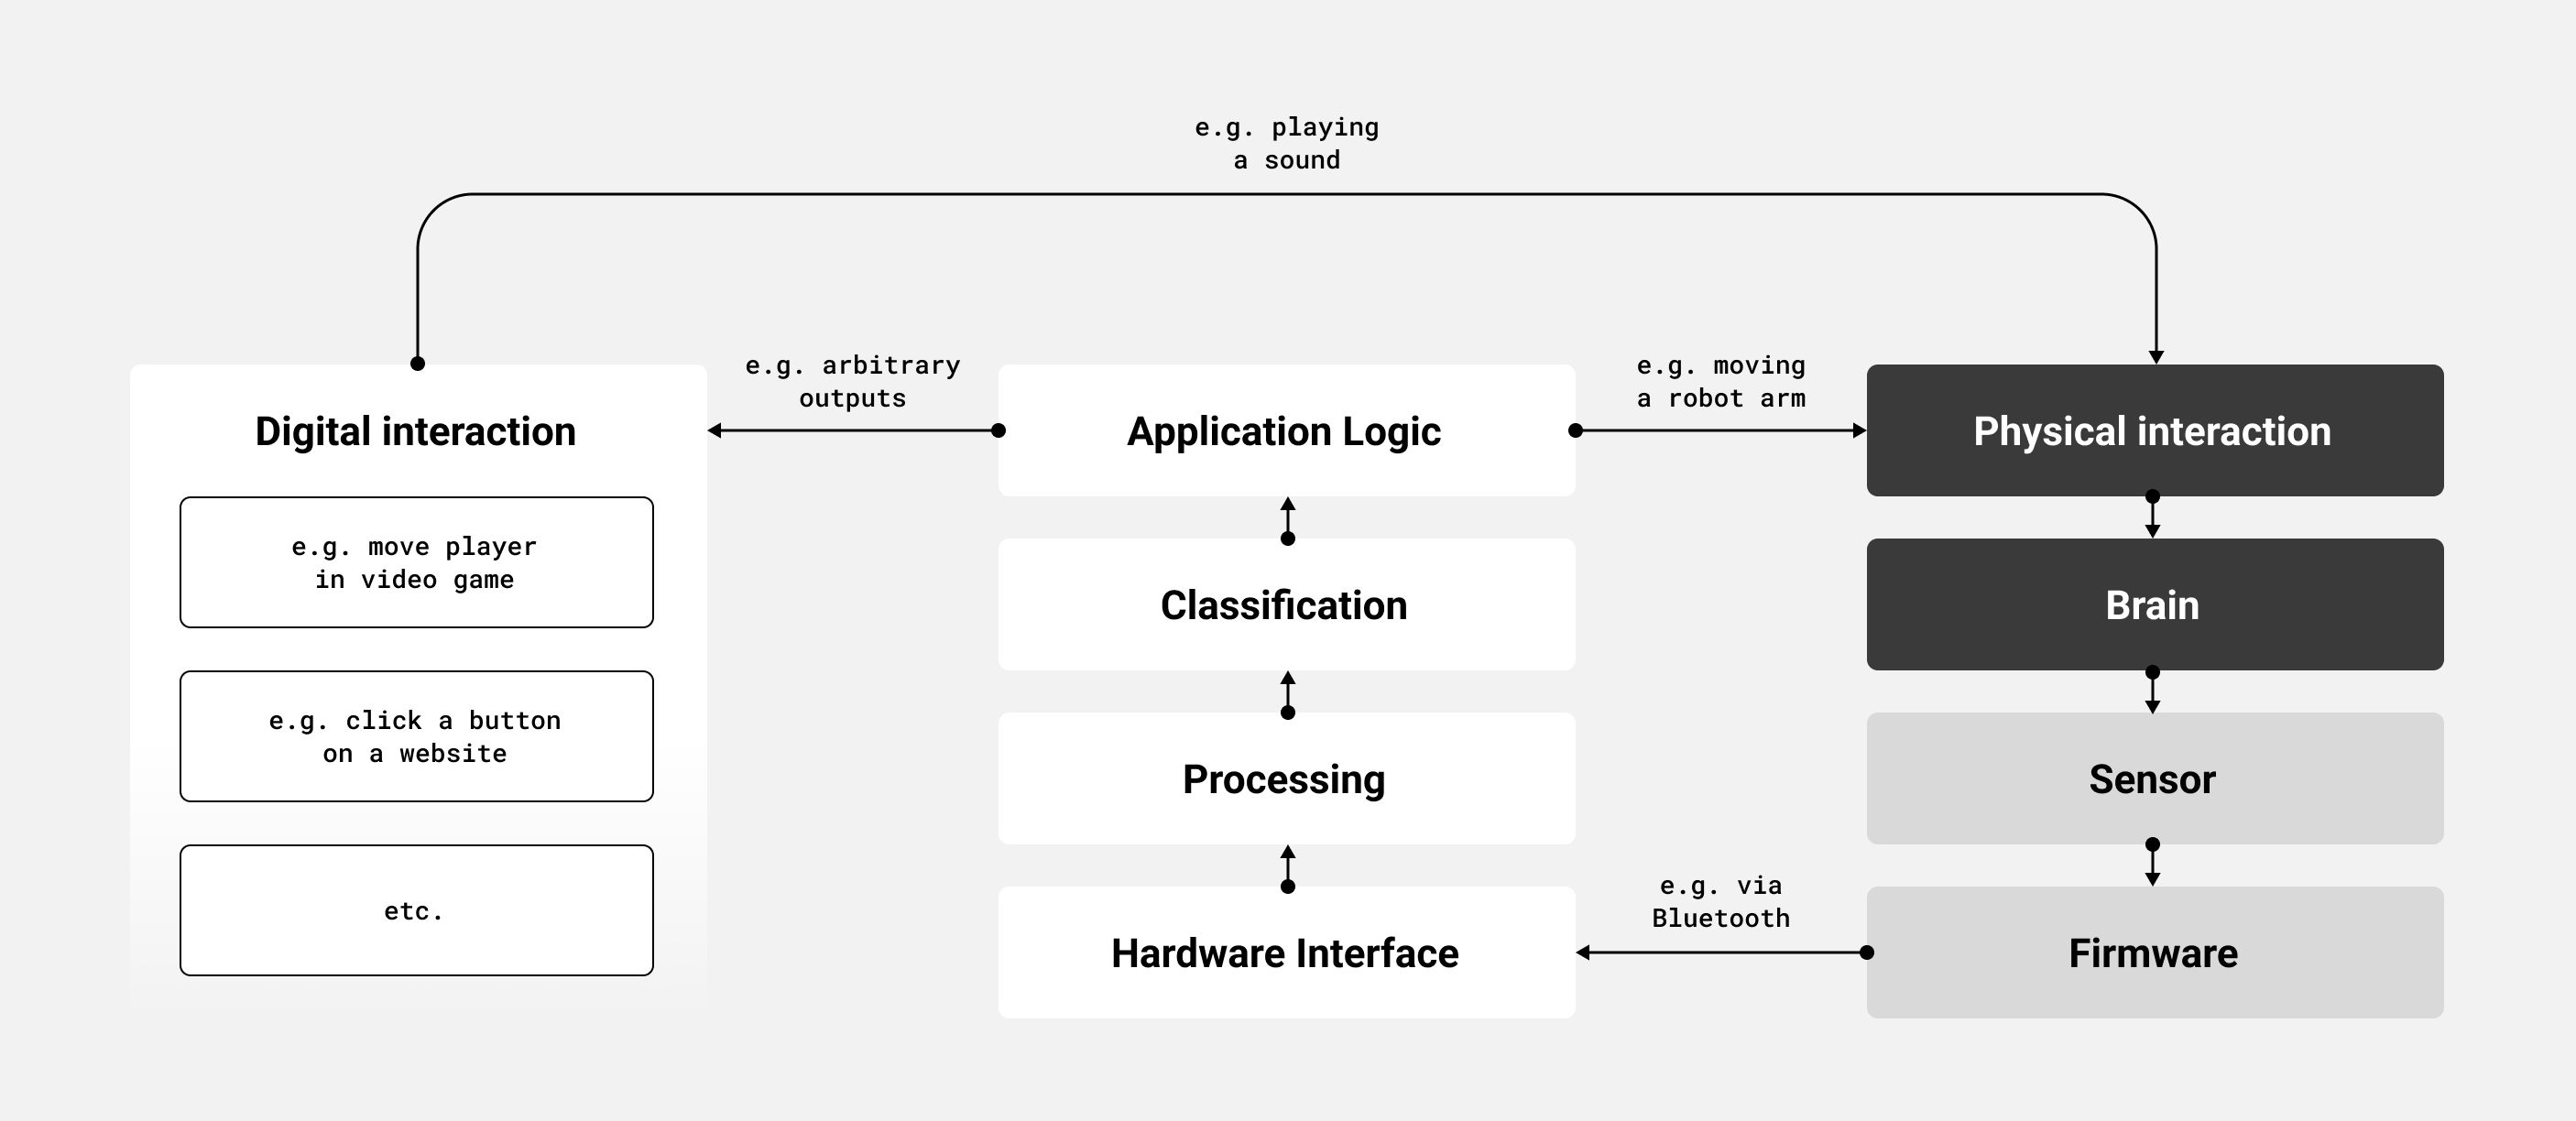
\includegraphics[width=\linewidth]{bci-components.png}
  \caption{Architectural overview of BCI components including a bidirectionality due to neurofeedback in form of e.g. playing a sound in a certain frequency to enable SSVEP}
  \label{fig:bci-components}
\end{figure}

 The application layer, as shown on \autoref{fig:bci-components} is the part of a BCI that gets the interpreted data from, e.g. a classification model and turns it into applicable functionality to interface with a physical or digital counterpart to, e.g. move a player in a game or start playing sound on the computer via its speakers. There is also the physical part, e.g. the brain and a physical interaction counterpart in the form of, e.g. a robot arm. The totality of the software stack is responsible for processing the data, e.g. extracting the relevant information from the raw data and turning it into any desired and meaningful output for the application layer.

\subsection{Unobtrusive hardware and software}
\label{chapter2-unobtrusive-hardware-and-software}

The unobtrusiveness of hardware and software is another aspect to consider when discussing BCIs. Unobtrusiveness in hardware means that it is either not visible at all\footnote{There are other things related to the overall user experience (UX) that are sometimes included in the notion of unobtrusiveness, such as comfort, reusability and convenience, where the author only implies physical characteristics such as shape and size}, such when sensors are implanted beneath the skull, or that it is in a form factor that is already socially established.

\begin{figure}[!ht]
  \minipage{0.49\textwidth}
  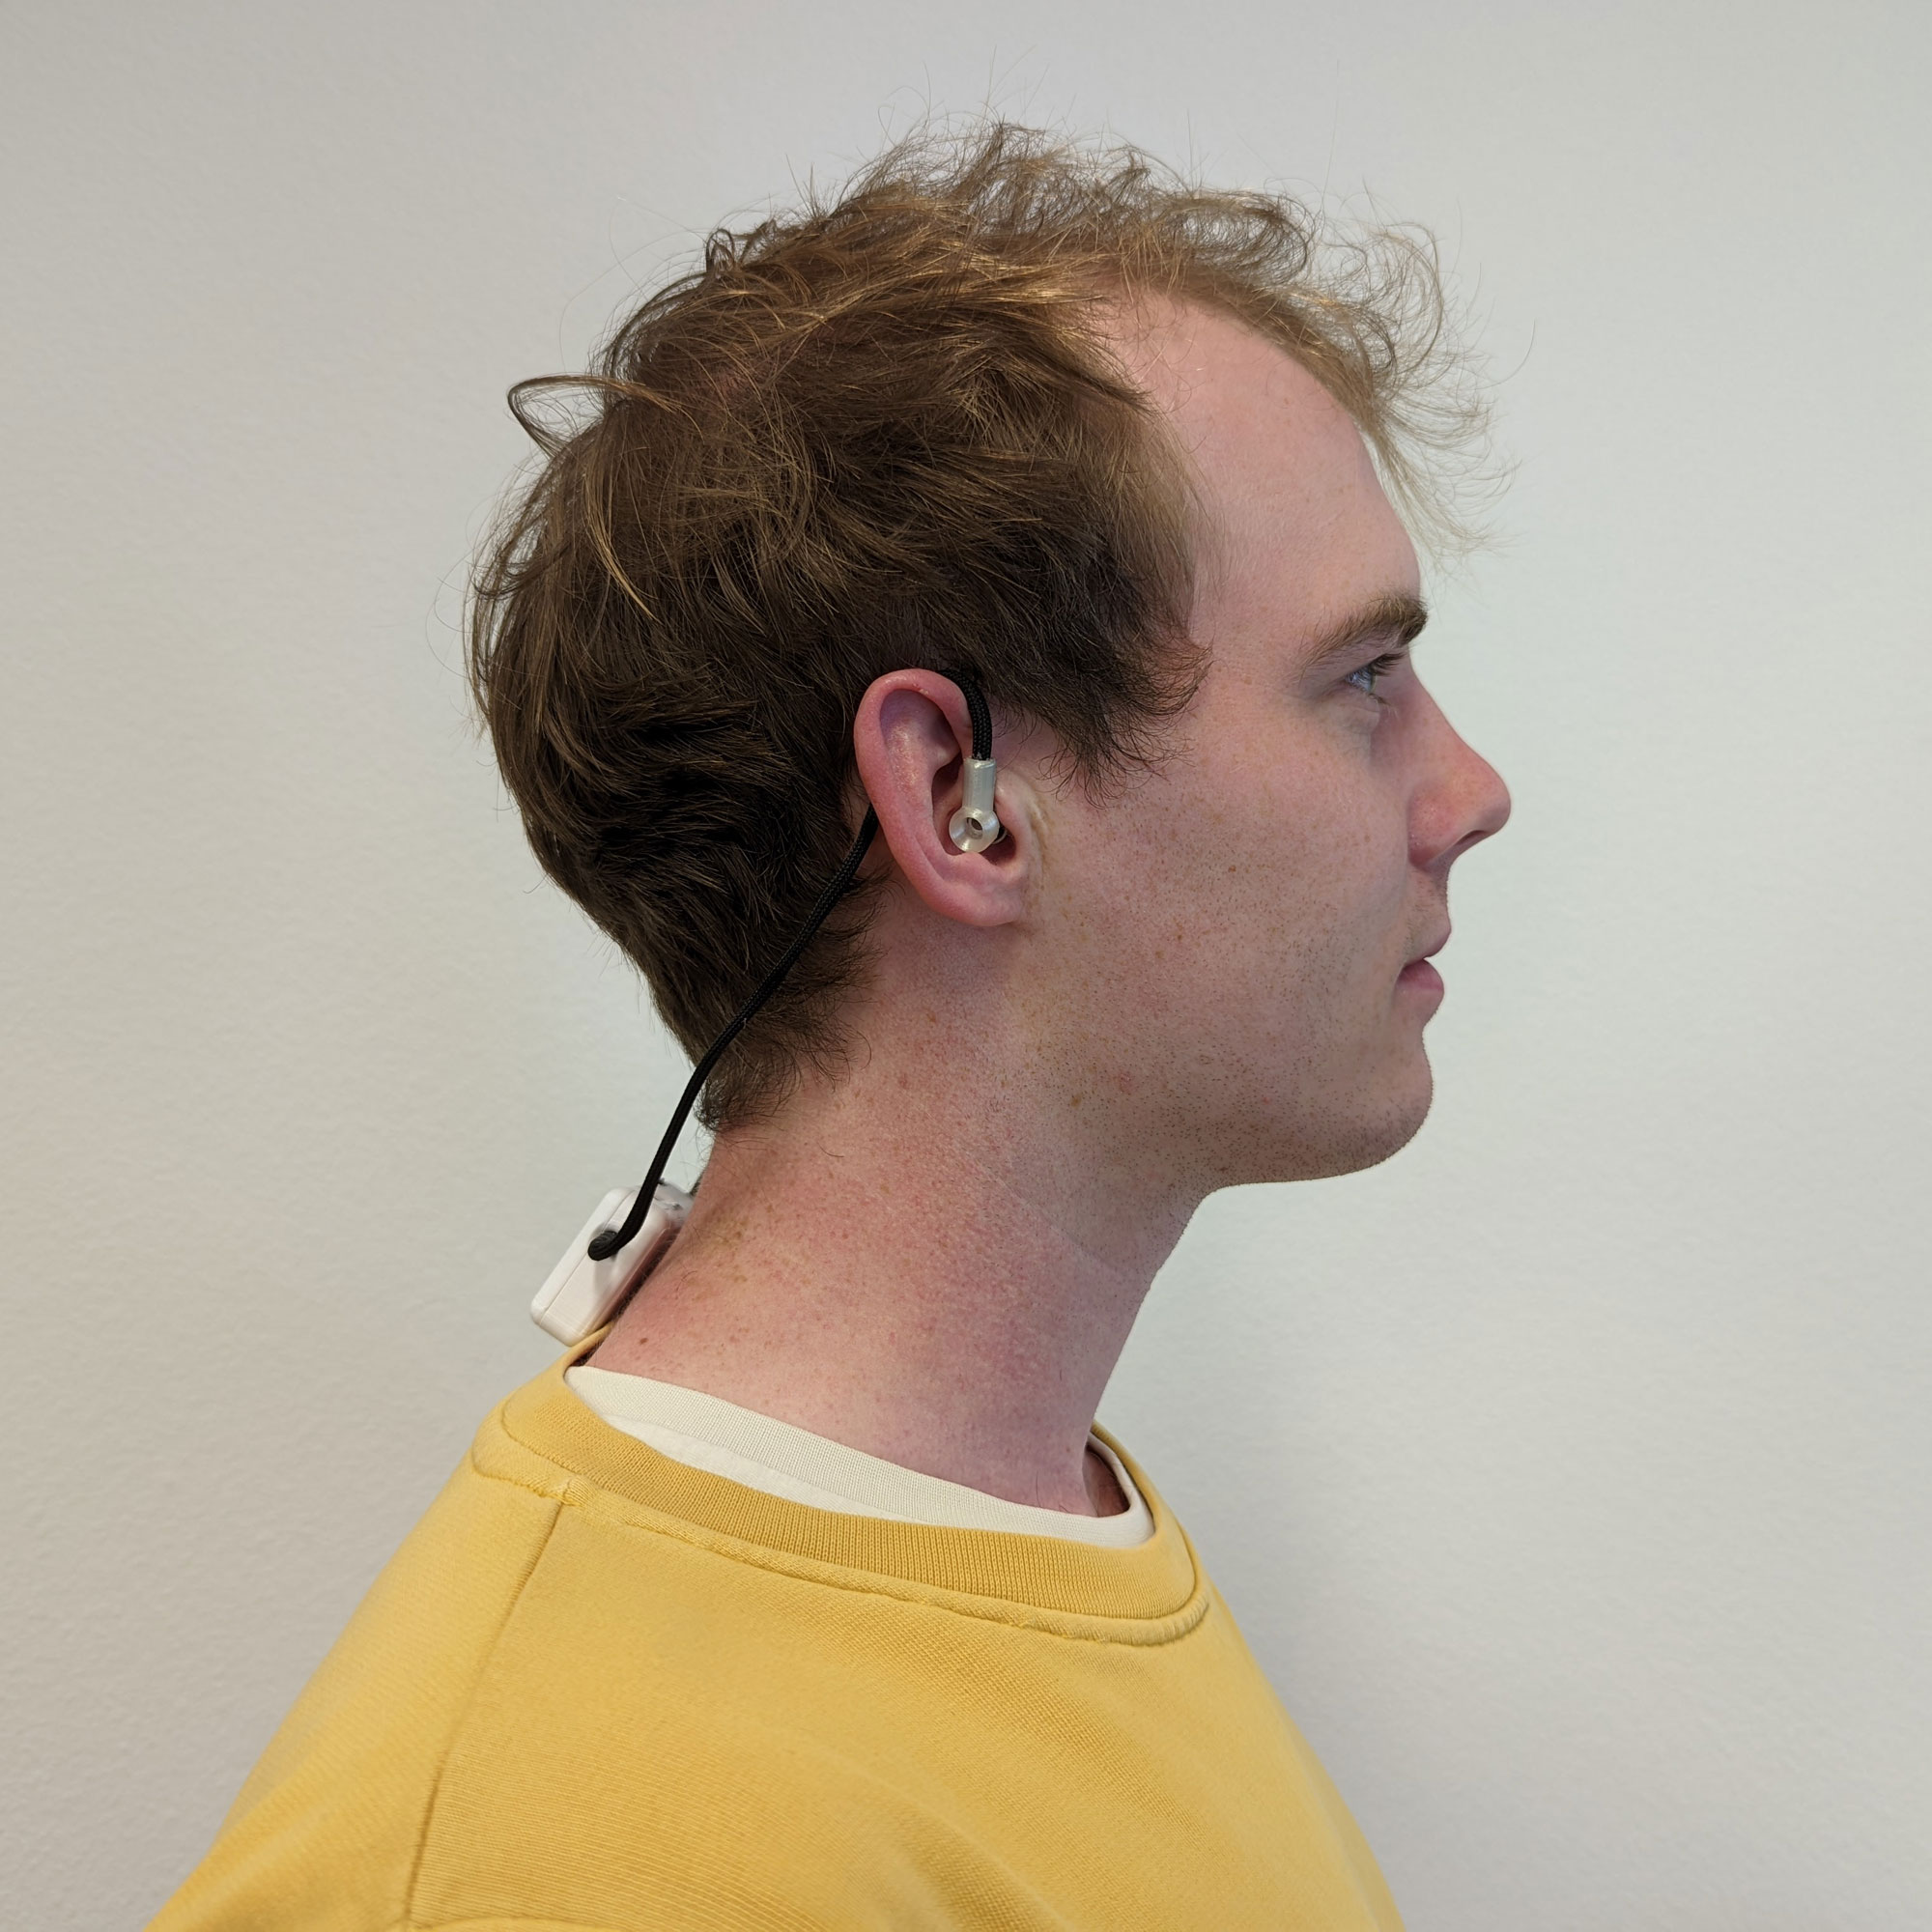
\includegraphics[width=\linewidth]{unobtrusive.jpg}
  \caption{IDUN Guardian hardware, \\ unobtrusive BCI}
  \label{fig:unobstrusive-hardware}
  \endminipage\hfill
  \minipage{0.49\textwidth}
  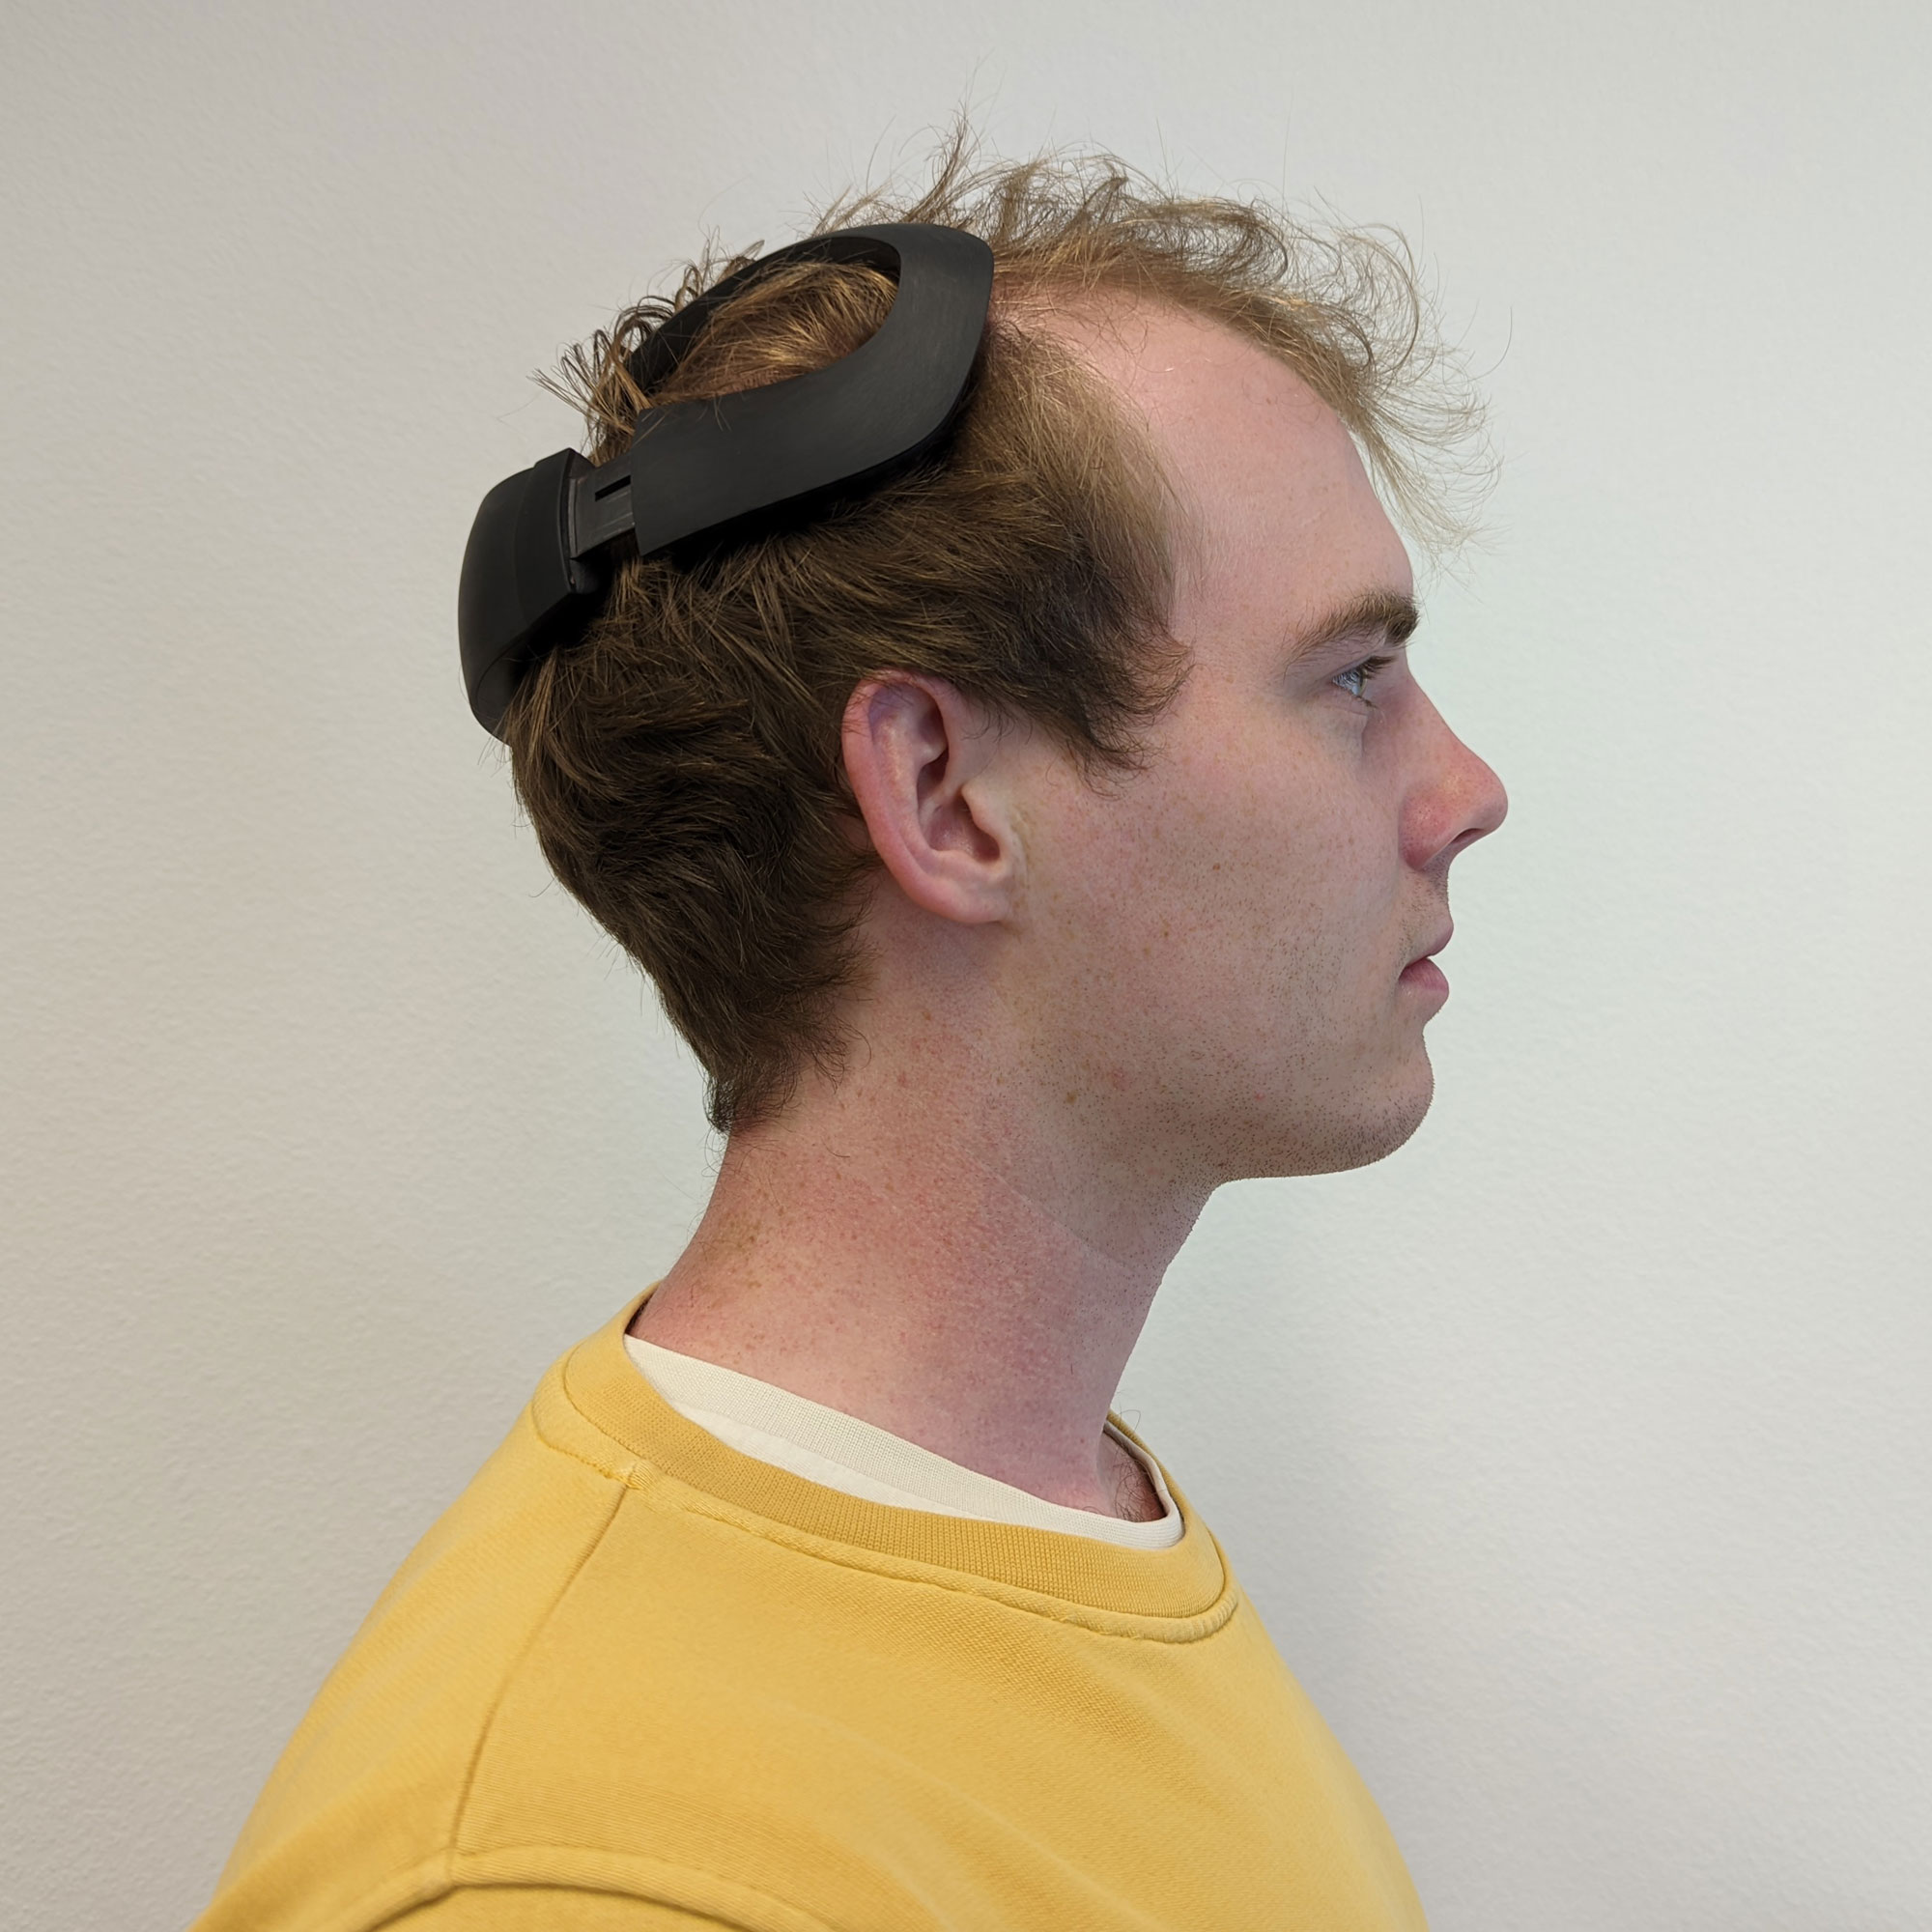
\includegraphics[width=\linewidth]{obtrusive.jpg}
  \caption{Neurosity Notion hardware, \\ obtrusive BCI}
  \label{fig:obstrusive-hardware}
  \endminipage\hfill
\end{figure}

The prototype of, e.g. IDUN Technologies' hardware, as shown in \autoref{fig:unobstrusive-hardware} measures brain activity in the ear canal that aims to resemble the form factor of established in-earbuds. \autoref{fig:obstrusive-hardware} shows the Notion device from Neurosity, which measures EEG on the head and is not comparable to a socially established form factor such as earbuds.

What is considered socially established and accepted truly depends on the society and context, as one could argue that wearing a Neurosity device under a hat while talking to a friend is more acceptable than wearing in-earbuds. Still, the implications of different form factors must also be considered, such as the possibility of moving the device and thus creating motion artefacts in the signals or the position of the sensors. The ear canal, for example, is ideally closely located to the brain's auditory cortex but not so much for the visual cortex, which is located at the back of the head. However, further hardware implications for BCIs are not a topic covered in this thesis.

Furthermore, it is perhaps not as simple to discuss the unobtrusiveness of software as it is with hardware. Unobtrusive\footnote{Other words for unobtrusive could be discreet, fully-integrated, invisible or simply "in the background".} software, as defined by the author, is the abstraction of the underlying software or system that executes the logic to fulfil a task without the user knowing what the technical requirements are. As an example: To use an HP ENVY Photo 6200 printer with one's Android phone, one must first download the HP Smart app and the HP Print Service Plugin app that acts as a driver for the printer in order to get it set up and running \citep{hp_hp_nodate}. In the case of the HP printer, the user must understand some of the underlying technical requirements in order for it to work, rather than simply concentrating on the task of printing something. For example, unobtrusive software is when one gets a new computer mouse that they simply plug in and it works\footnote{Unobtrusiveness usually correlates with usability, but it is not always the case, e.g. more advanced users would not consider locked-in abstraction as more usable.}.

Unobtrusive software in BCI refers to the ability to connect one's hardware to the computer or smartphone and use it without the need for additional software such as drivers or command-line interface (CLI) software. As an example: To use an OpenBCI device, one needs to open the GUI app, connect the hardware, presumably test its quality, begin a data stream session, and output the stream via a network protocol such as a Lab Streaming Layer (LSL), connect to the signal from, e.g. Neuromore Studio \citep{openbci_neuromore_nodate}, run the data through a classification pipeline, and then connect the output from Neuromore to a video game via the engine itself to have controls for the video game. It should go without saying that this is not unobtrusive software. There are examples of software that is included as an executable file and thus is relatively unobtrusive, but the software is closely linked with the hardware and the brand behind the hardware, or it is in the proof of concept (PoC) stage rather than a production-ready application. Buying a new pair of headphones and plugging them into one's computer to enjoy neuro-enhanced\footnote{Neuro-enhanced software can be described adding additional features to input methods via the brain.} experiences interacting with the brain's outputs or measuring brain data across all apps and the operating system would be an example of proper unobtrusive BCI software.

\subsection{Production-grade software}
\label{chapter2-production-grade-software}

There is no clear definition of what production-grade software is, but in most cases, software developers agree on the following points:

\begin{itemize}
  \item The software works at any time when access is required. It is therefore capable of frequent and intensive use in, e.g. commercial or industrial environments.
  \item Software whose behaviour is deterministic and predictable and is, therefore, well-tested, well-documented and optimised in terms of speed, efficiency and security for the given context (e.g. the size of the user base). Usually, developers agree on a Definition of Done (DoD) inside their team to what is considered production-ready, e.g., test coverage of 80+\%, peer-reviewed and commented code, and a common code style guide, to name a few.
  \item Software that runs in a production environment, i.e. on a cloud computing cluster for actual users rather than in a test environment for test users or, for example, on hardware delivered to real customers, and that can adapt itself to the context, e.g. to a higher access rate or insecure user-generated input. In most cases, especially in cloud computing, production-grade also means larger data sets, such as in databases, the possibility of a more significant number of edge cases due to a larger user base, and, most importantly, more available computing power on production instances.
\end{itemize}

As stated in previous sections, most BCIs, such as the OpenBCI, are not intended for production. They are intended for PoCs used in examples, such as controlling objects in games or conducting simple research. End-to-end and full-stack BCIs for production are rare, as most are very specific and not intended for general purposes, such as the Muse headband, or the software aspect is intended for PoCs or research, such as with, e.g. Emotiv, another BCI company from the USA. Pure software products, such as Neuromore, lack the hardware component and miss, for example, an SDK that can be integrated into existing software for different platforms. Neurosity, for example, aims to provide a universally usable and unobtrusive software stack that is even open-source. However, because the hardware is not unobtrusive enough, it does not qualify the author's definition as production-grade (apart from the fact that it is not known whether their software stack is aimed to be used in production \citep{neurosity_neurosity_2022} due to, e.g. third-party developers providing disclaimers of being a work in progress \citep{turney_notion_2022}). Companies such as e.g. Neuralink are presumably working on a general-purpose, unobtrusive and production-ready software system which enables developers to build production apps and even platforms on top of it for a variety of use cases without being limited \citep{musk_integrated_2019}, in their case, since it is a bidirectional BCI, developers are also able to write data back to the brain. Since their aimed hardware is also as unobtrusive in the form factor (since it is implanted), they have a high potential to become one of the first mass-market-ready BCIs if we ignore the fact that we need surgery to get the device itself \citep{neuralink_approach_nodate} and other considerations as a harder opt-out of the device compared to, e.g. plugging out earphones.

\section{Neural/cloud interface definition}
\label{chapter2-neural-cloud-interface-definition}

This section discusses the definition, need and differentiation of a N/CI and the paradigm shifts associated with it when discussing BCI software.

\subsection{BCI software on the cloud}
\label{chapter2-bci-software-on-the-cloud}

Looking at \autoref{fig:nci-components}, we can see that the three software layers of a BCI-component illustration, as pictured on \autoref{fig:bci-components} are highlighted. This is because these components can run on the cloud, i.e. on a public cloud provider such as Amazon Web Services (AWS).

\begin{figure}[ht]
  \centering
  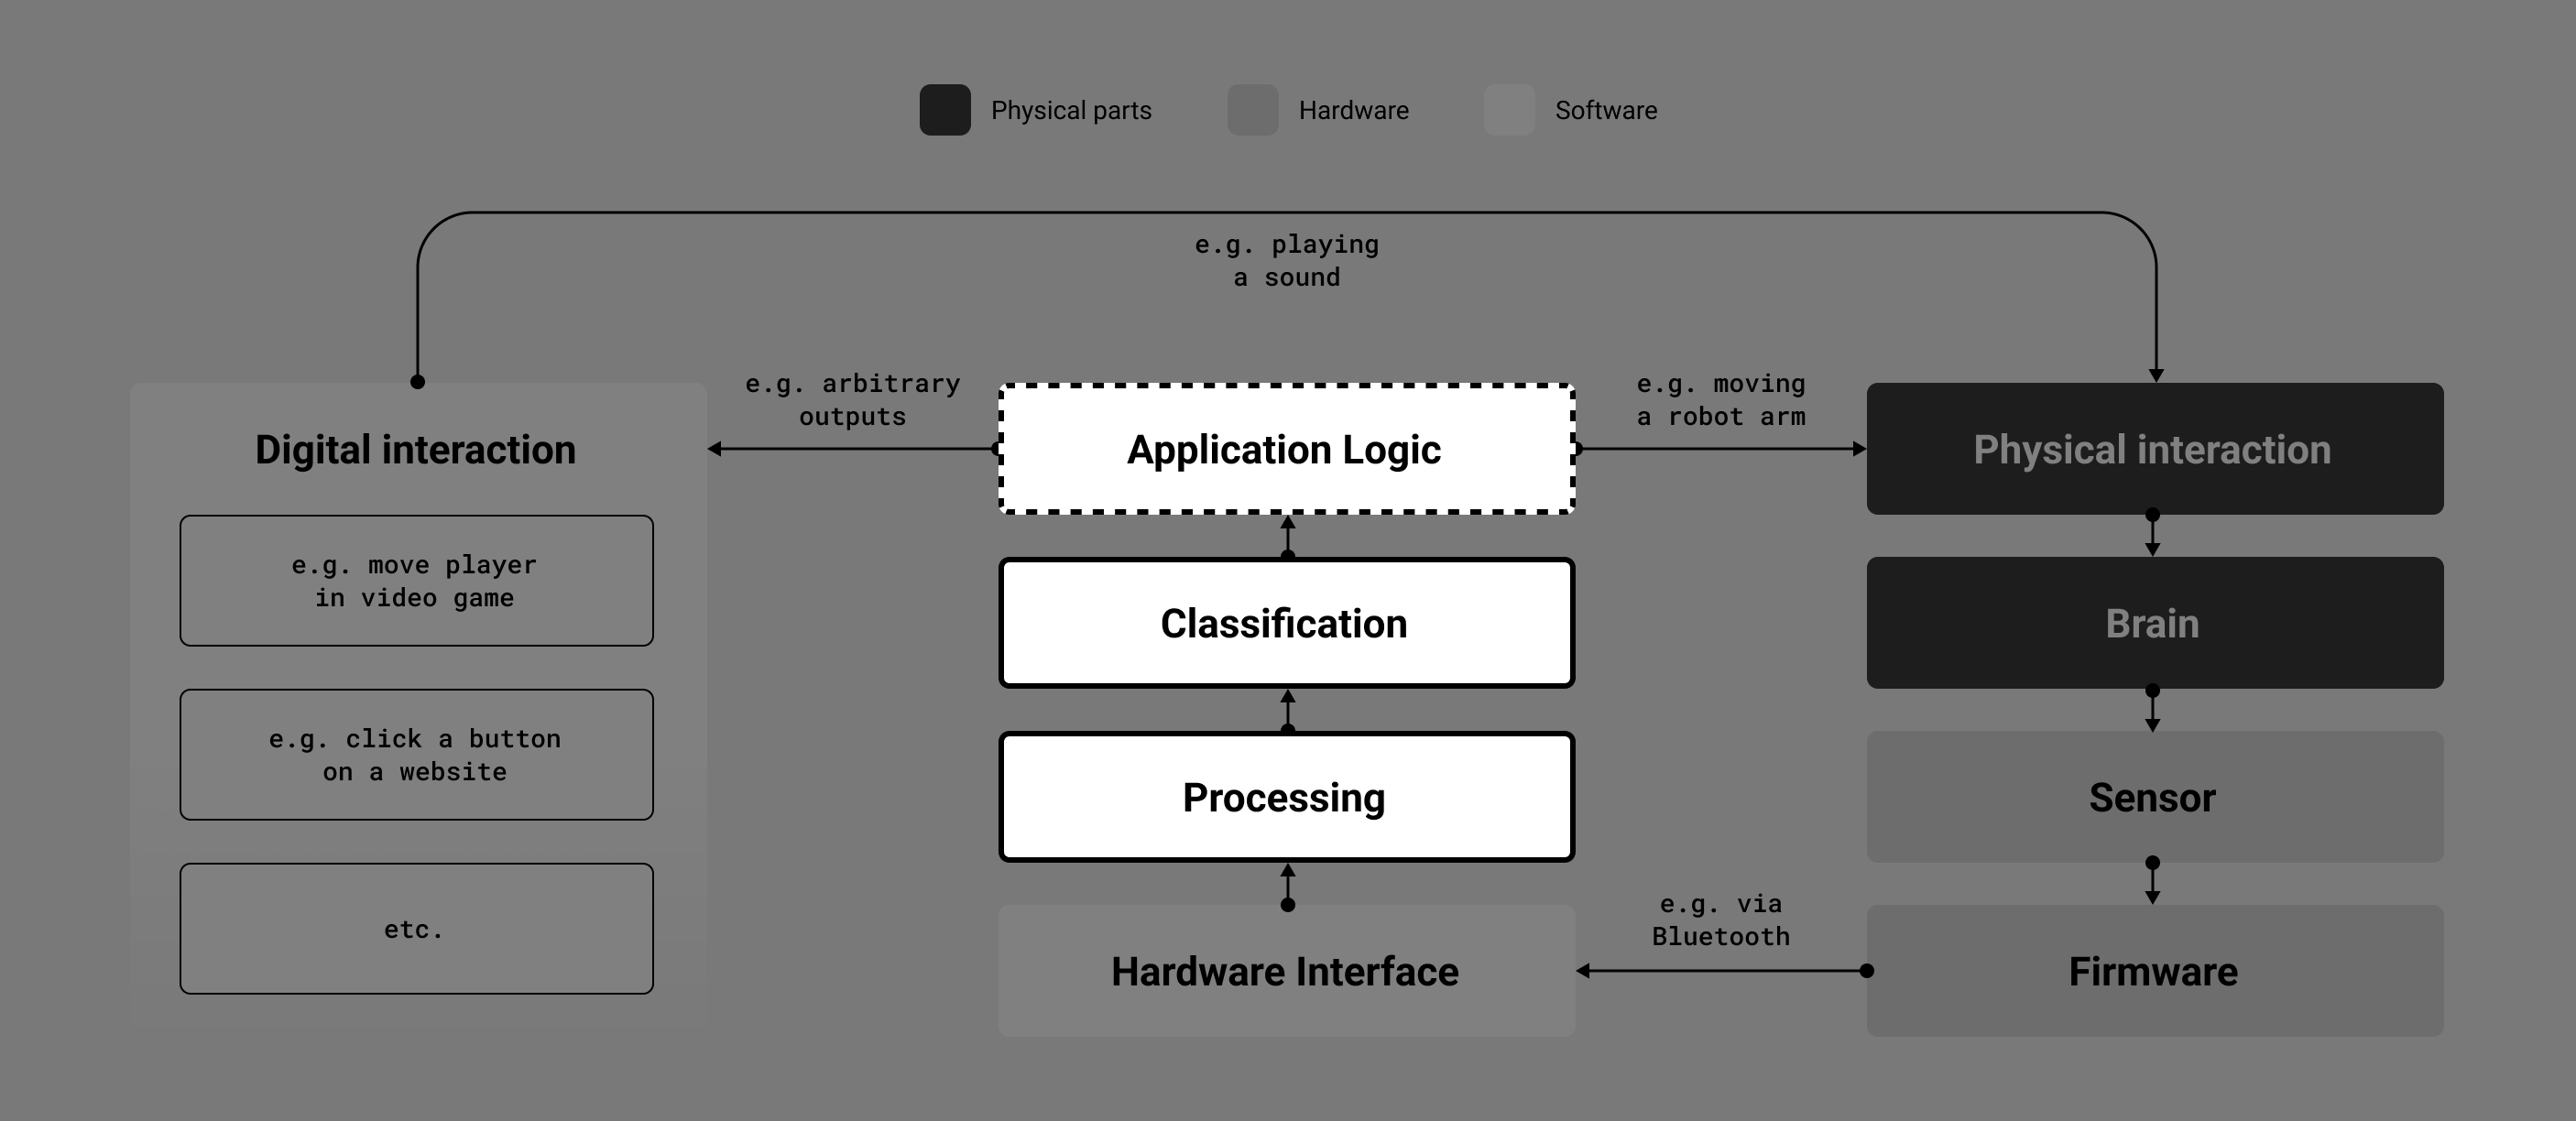
\includegraphics[width=\linewidth]{nci-components.png}
  \caption{Highlight of the software components as shown on \autoref{fig:bci-components} of a BCI that could be moved to the cloud.}
  \label{fig:nci-components}
\end{figure}

Running software on the cloud means that developers or companies can access provisioned information technology (IT) infrastructure through the internet, usually with a pay-as-you-go pricing model \citep{amazon_web_services_inc_what_nodate}. The development speed of software applications can drastically improve since software developers can only focus on software rather than incorporating the hardware and network aspect of setting up their server farms, therefore abstracting the hardware part away. What started with simple computers that can be rented on a server such as it was with, e.g. AWS Elastic Compute Cloud (EC2) \citep{barr_amazon_2006} ended up being a diverse offering from cloud providers with various abstraction levels as shown on \autoref{tab:cloud-computing-types}.

\begin{table}[!ht]
  \centering
  \resizebox{\textwidth}{!}{%
    \begin{tabular}{ll}
      \rowcolor[HTML]{000000}
      {\color[HTML]{FFFFFF} Type}                                                                                 &
      {\color[HTML]{FFFFFF} Description}                                                                                                                                                                                                                                                                                                                           \\ \hline
      \multicolumn{1}{|l|}{\textbf{\begin{tabular}[c]{@{}l@{}}Infrastructure as\\ a Service (laaS)\end{tabular}}} &
      \multicolumn{1}{l|}{\begin{tabular}[c]{@{}l@{}}IaaS gives access to data storage space, virtual or dedicated\\ computers, and network services. The greatest degree of\\ flexibility and administrative control over your IT resources\\ are provided by utilising IaaS.\end{tabular}}                                                                       \\ \hline
      \multicolumn{1}{|l|}{\textbf{\begin{tabular}[c]{@{}l@{}}Platform as a\\ Service (PaaS)\end{tabular}}}       &
      \multicolumn{1}{l|}{\begin{tabular}[c]{@{}l@{}}PaaS lets developers concentrate on developing and\\ managing their code rather than worrying about the\\ underlying infrastructure (often hardware and operating\\ systems). An example is Kubernetes.\end{tabular}}                                                                                         \\ \hline
      \multicolumn{1}{|l|}{\textbf{\begin{tabular}[c]{@{}l@{}}Software as a\\ Service (SaaS)\end{tabular}}}       &
      \multicolumn{1}{l|}{\begin{tabular}[c]{@{}l@{}}SaaS provides a whole product that is run and controlled \\ by the service provider. The phrase SaaS often refers to\\ end-user apps (e.g. web-based email). Developers don't\\ have to be concerned about how the service is handled\\ or whether the underlying infrastructure is maintained.\end{tabular}} \\ \hline
    \end{tabular}%
  }
  \vspace{10pt}
  \caption{The three abstraction levels and types of cloud computing \citep{amazon_web_services_inc_what_nodate}.}
  \vspace{-5pt}
  \label{tab:cloud-computing-types}
\end{table}

The majority of businesses are anticipated to embrace a cloud-first strategy by 2025, according to Milind Govekar, vice president of IT research and consultancy company Gartner, and will not be able to fully implement their digital plans without the usage of cloud-native architectures and technologies \citep{gartner_gartner_nodate}. The impact and importance of cloud computing cannot be underestimated, and its success is also reflected in the annual spending on cloud computing resources, estimated at €474 billion in 2022 \citep{gartner_gartner_nodate}. Cloud computing is such an extensive and complex topic that it could quickly fill entire books. In the following list, the author categorises three essential points from a bird's eye view that certainly plays a vital role in BCI software: 1. Dedicated and deterministic environments, which explains that an environment of a software programme always stays the same independent of the end-users hardware, 2. elastic and high-performance availability, which explains cloud computers that have an on-demand and adjustable high-performance and 3. provided services for speed, which explains the concept of pre-made and dedicated software written primarily for the cloud and specific use cases. The following list goes more into detail about the mentioned topics in the context of BCI software:

\begin{itemize}
  \item \textbf{Dedicated and deterministic environments:} Running code for BCIs on different end-user platforms, such as Windows or Android, can have drawbacks because each device has its processor, graphics card, operating system version and drivers, which can make developing software that requires stable and good performance, such as a neural data processing pipelines, time-consuming and difficult to maintain, as developers must keep track of every factor of the end-user devices. This is fine for BCIs that are not intended for the general public, such as specially designed BCIs for people with, say, locked-in syndrome, but for the general public, a variety of different end-user devices come into play. When code is run on a dedicated machine, such as a cloud computer with clearly defined hardware and operating system specifications, it becomes less error-prone and more deterministic.
  \item \textbf{Elastic and high-performance availability:} Because the cloud model usually runs as an as-needed model, the initial purchase cost of computer hardware is split and shared across usage. Developers have access to tremendous computing power that would not be easily afforded if purchased independently. As a result, when developing a computationally intensive algorithm, developers can use high-performance central processing units (CPUs) and graphics processing units (GPUs) to complete tasks much faster than consumer hardware on end-user devices. Performance can also be increased as needed, for example, to handle heavier tasks that are not used as frequently or to handle more requests when, for example, the demand for the software increases due to an increase in the number of users, which is a process known as elasticity \citep{gartner_definition_nodate}. Furthermore, the cloud provides far more storage capacity than end-user devices.

  \item \textbf{Provided services for speed:} The vast majority of cloud providers are providing more specialised services as we move closer to PaaS. Provisioned database servers, for example, exist solely to serve as a database, so the underlying hardware is optimised for the database software running on it, such as, e.g. PostgreSQL. Hundreds of cloud computing services are available, including 200 from AWS alone \citep{amazon_web_services_inc_what_nodate}, all of which address specific use cases. This is extremely useful when it comes to cloud-based BCI software. One example is the aspect of live streaming of brain data, which we will go over in greater detail in the implementation chapter of this thesis. The services provided accelerate development by eliminating the need for teams to reinvent the wheel repeatedly, and they also provide out-of-the scalability, such as in the serverless model \citep{redhat_what_2022}.
\end{itemize}

A N/CI utilises cloud computing by running certain software components of a BCI system in the cloud as, e.g. shown on \autoref{fig:nci-components}. Multiple BCIs can communicate with each other or with other software or hardware over the internet, enabling remote HCI. \autoref{fig:nci-overview} depicts how two or more BCIs can interface with one another using cloud software. The red arrows represent the typical local BCI. The blue arrow depicts how the person on the left can execute business logic via the cloud over the internet, enabling digital and physical interactions with, e.g. high performance. The green arrow depicts how the person on the right can communicate with their BCI via a N/CI with the person on the left even if they are not in the same geographical location.

\begin{figure}[ht]
  \centering
  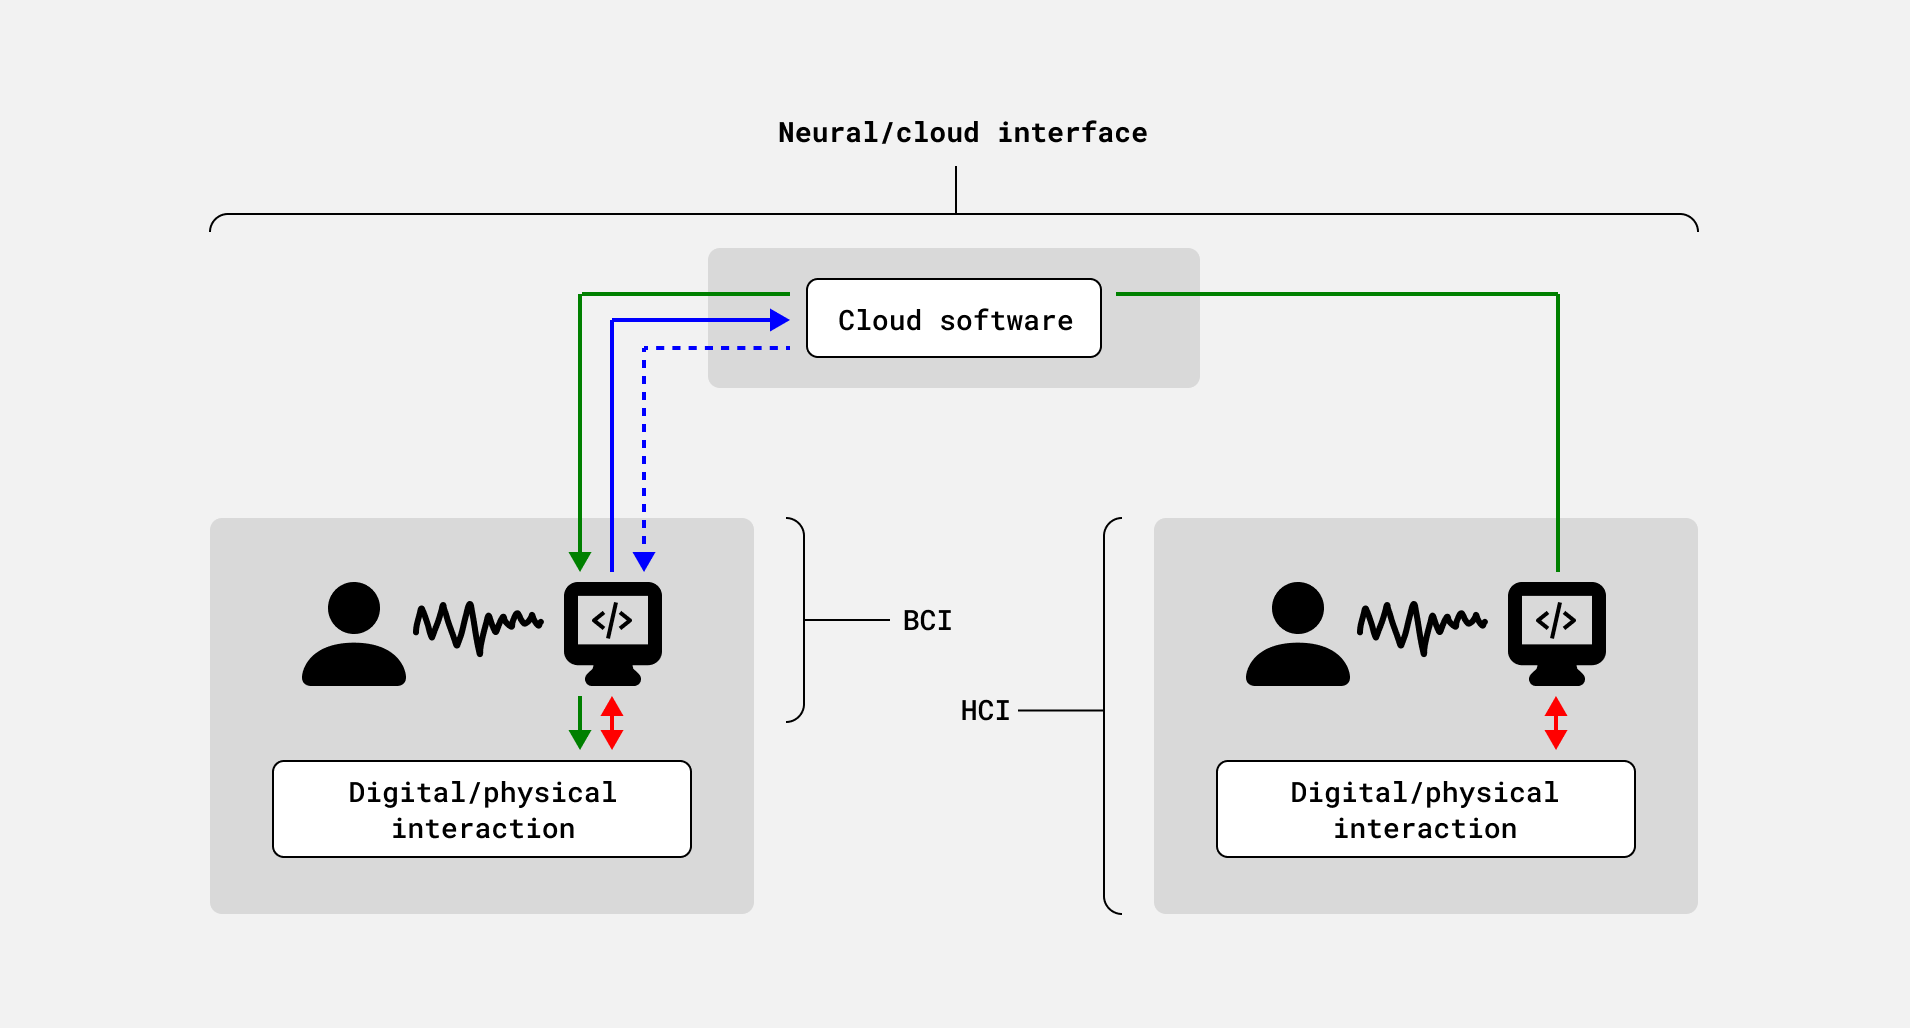
\includegraphics[width=\linewidth]{nci-overview.png}
  \caption{A N/CI is the connection between multiple BCIs}
  \label{fig:nci-overview}
\end{figure}

\subsection{Distinction between existing research}
\label{chapter2-distinction-between-existing-research}

The concept of running BCI software components remotely and on servers is not new and novel, as research into the concept known as asynchronous BCI \citep{an_design_2016} or internet-based BCI \citep{lampe_brain-computer_2014} has been ongoing for some time. When we look at the research from, e.g. \citeauthor{zhang_internet_2018} from 2018 on their deep learning framework to enable as they describe Human-Thing Cognitive Interactivity, we see a strong emphasis on algorithms and machine learning but less on aspects such as cloud architecture and production-readiness \citep{zhang_internet_2018}. They address the latency and the size of EEG samples sent in real-time to a server, as well as the corresponding calculation, but there are no more details in regards to the proposed and very simplified architecture chart's protocols and effective cloud architecture, all of which factor into the author's task to develop a N/CI system. Another paper by \citeauthor{ahamad_system_2022} looks at the system architecture of a BCI for the Internet of Things (IoT), but this time from the perspective of algorithms optimised for time series data such as EEG, with no mention of the effective cloud architecture of such a system \citep{ahamad_system_2022}.

The author of this thesis introduces the concept of three-dimensionality for the definition of a N/CI based on the previously mentioned topics and research that touch on the issues of this thesis, which are essential to achieve mass adoption for BCIs from the perspective of the software system for the actual implementation of such a system.

\subsection{Requirements of a N/CI}
\label{chapter2-requirements-of-a-nci}

The term N/CI positions itself as a software system in the intersection that can undoubtedly be defined as production-grade rather than being in the PoC stage, unobtrusive implementation rather than obtrusive software and general-purpose applicability rather than being made just for a specific use case. \autoref{fig:nci-definition} illustrates the position of a N/CI within the mentioned properties. Subsequently, \autoref{tab:nci-axis} summarises the definitions as described in this thesis.

\begin{figure}[ht]
  \centering
  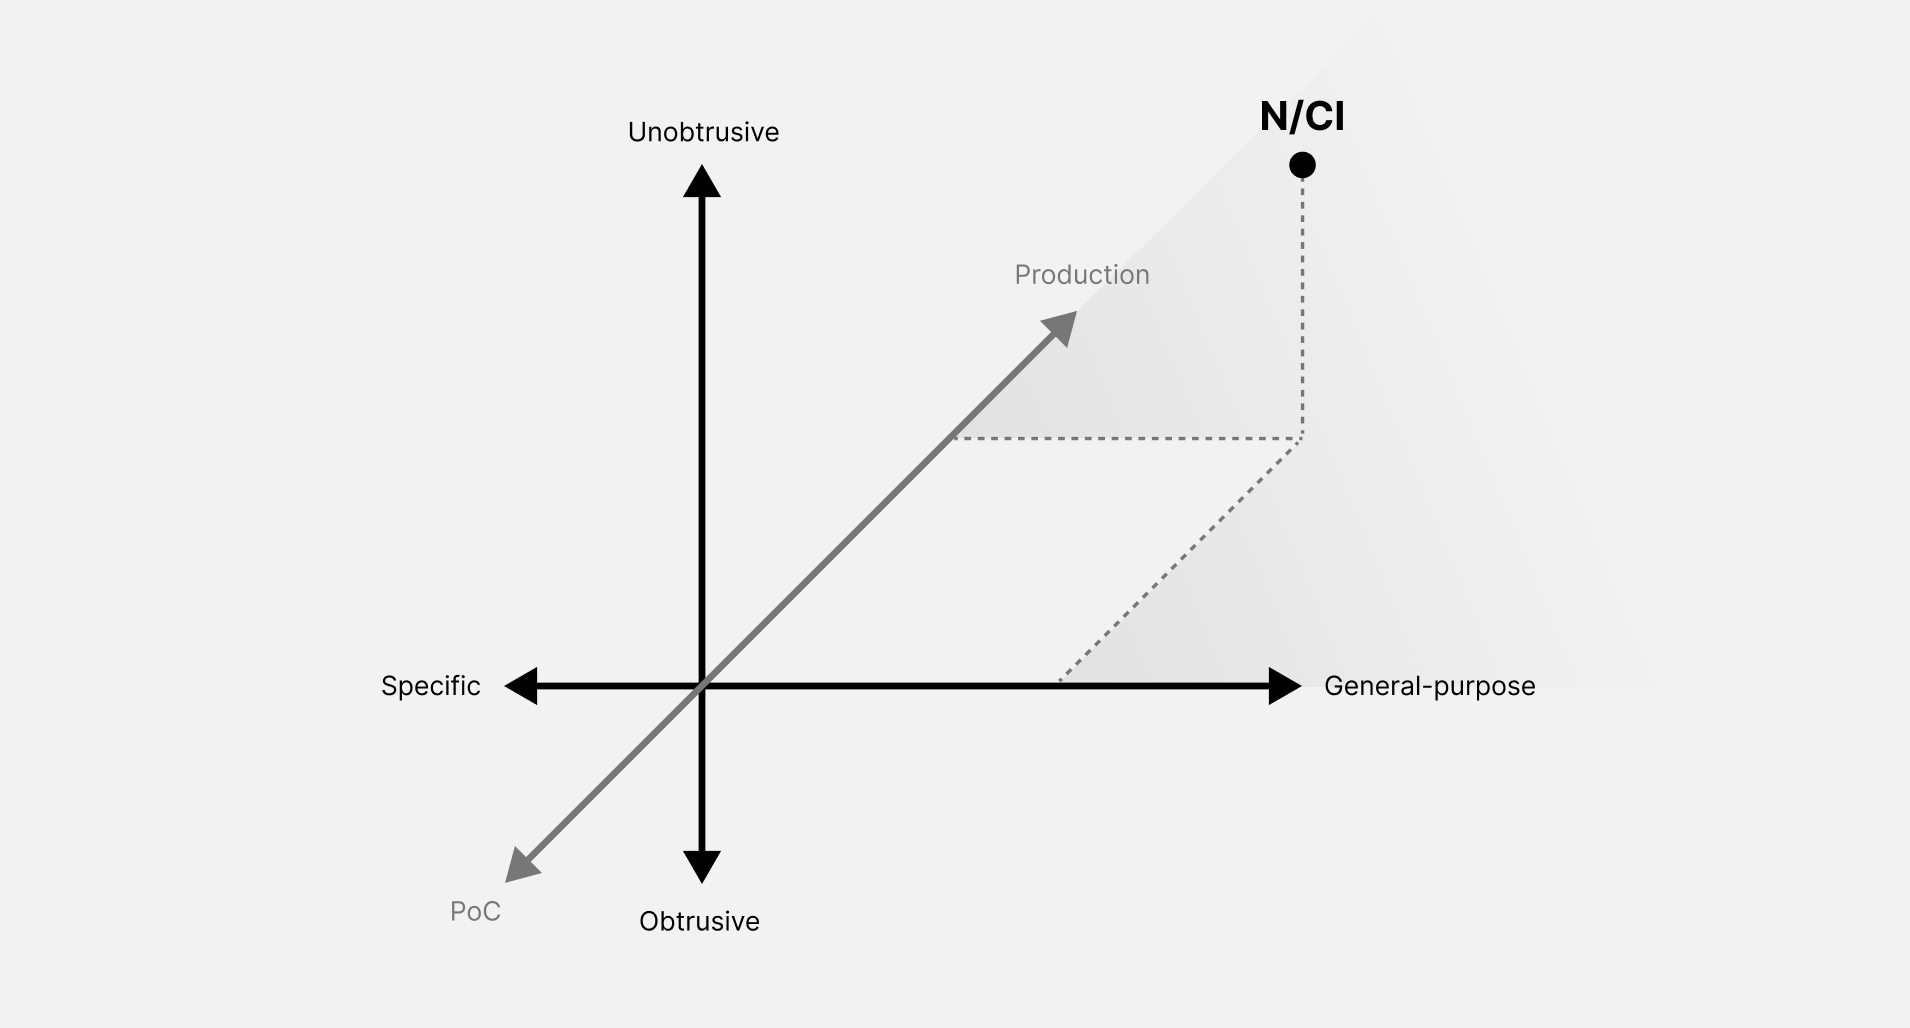
\includegraphics[width=\linewidth]{nci-definition.png}
  \caption{Visualisation of the three-dimensionality of the term neural/cloud interface with its three axes and differentiation of six terms}
  \label{fig:nci-definition}
\end{figure}


\begin{table}[ht]
  \centering
  \resizebox{\textwidth}{!}{%
    \begin{tabular}{ll}
      \rowcolor[HTML]{000000}
      {\color[HTML]{FFFFFF} Axis labelling}                   &
      {\color[HTML]{FFFFFF} Description}                                                                                                                                                                                                                                                                                                                                                                                                                                                                                                                                                                                  \\ \hline
      \multicolumn{1}{|l|}{\textbf{Production}}               &
      \multicolumn{1}{l|}{\begin{tabular}[c]{@{}l@{}}As previously stated, this is the range in which a software system is deemed ready for production.\\ Because the definition is vague, it is difficult to identify specific requirements that must be met for\\ a system to be considered production-ready. However, for a N/CI, this means running in a\\ production environment, e.g. in a cloud, on a real-world end-user server rather than, for example,\\ in a proof-of-concept environment such as in a lab.\end{tabular}}                                                                                     \\ \hline
      \multicolumn{1}{|l|}{\textbf{Unobtrusive}}              &
      \multicolumn{1}{l|}{\begin{tabular}[c]{@{}l@{}}As previously stated, an unobtrusive software system is one in which the end-user does not need\\ to understand the underlying architecture and requirements in order to use the software or even\\ know certain parts of the software system. In the reverse case, users need to install special\\ packages or download additional companion apps. to make a N/CI work on their computer\\ or smartphone is not the aim of the author's definition of a N/CI.\end{tabular}}                                                                                         \\ \hline
      \multicolumn{1}{|l|}{\textbf{General-purpose}}          &
      \multicolumn{1}{l|}{\begin{tabular}[c]{@{}l@{}}A general-purpose software system is one that can be used for a variety of functions. As an\\ example, consider AWS. It is general-purpose, which means that developers can create\\ cloud software on AWS that can be either a financial application or a backend for a mobile\\ application; there are no specific use cases. This means that a N/CI, unlike the NextMind BCI\\ or the Muse headband, should provide general-purpose functionality rather than specific use\\ cases, i.e. it is not limited to a specific set of functions.\end{tabular}}          \\ \hline
      \rowcolor[HTML]{EFEFEF}
      \multicolumn{1}{|l|}{\cellcolor[HTML]{EFEFEF}PoC}       &
      \multicolumn{1}{l|}{\cellcolor[HTML]{EFEFEF}\begin{tabular}[c]{@{}l@{}}A BCI software system that serves as a proof of concept cannot be considered N/CI because\\ it is not intended for production and thus all the effort required to create a production system,\\ such as quality assurance with unit or end-to-end testing, is unnecessary. A PoC system does\\ not usually run in a production environment, as the goal is, for example, to test a specific\\ functionality of a use case rather than to deliver the software to end-users.\end{tabular}}                                                    \\ \hline
      \rowcolor[HTML]{EFEFEF}
      \multicolumn{1}{|l|}{\cellcolor[HTML]{EFEFEF}Obtrusive} &
      \multicolumn{1}{l|}{\cellcolor[HTML]{EFEFEF}\begin{tabular}[c]{@{}l@{}}An obtrusive BCI system, for example, may still be production-ready if it targets specific use cases\\ while remaining unobtrusive because neuroscientists or developers, for example, expect to have\\ access to the underlying software architecture or technical requirements and thus do not want to\\ abstract from it. If it is obtrusive software, such as OpenBCI, this usually means building the\\ production-ready part on top of it is necessary, which does not fit the author's proposed definition\\ of a N/CI.\end{tabular}} \\ \hline
      \rowcolor[HTML]{EFEFEF}
      \multicolumn{1}{|l|}{\cellcolor[HTML]{EFEFEF}Specific}  &
      \multicolumn{1}{l|}{\cellcolor[HTML]{EFEFEF}\begin{tabular}[c]{@{}l@{}}If a BCI system is only used for one use case, such as Muse for sleep and meditation, companies\\ or developers who want to offer a different use case, such as a mind-controlled keyboard with a\\ P300 system will have to reverse engineer Muse's EEG output or use a different BCI hardware\\ that is less specific and closed, and then build their own production-ready and unobtrusive software\\ on top of it.\end{tabular}}                                                                                                         \\ \hline
    \end{tabular}%
  }
  \vspace{10pt}
  \caption{Axes label descriptions of the three-dimensionality for the definition of a N/CI as shown on \autoref{fig:nci-definition}}
  \label{tab:nci-axis}
\end{table}

\newpage

With an unobtrusive form factor like the one developed by IDUN Technologies, a significant hardware barrier to becoming a mass-market BCI has already been overcome. Next to the hardware, IDUN intends to provide a business-to-business (B2B) software platform, allowing third-party developers to create software on top of IDUN's offerings through a universal brain application programming interface (API). Because IDUN allows others to consume this API in end-user-facing apps, it must be production-ready and unobtrusively able to be implemented. IDUN's hardware and software should be general-purpose rather than specific, allowing developers to build any neuro-enhanced application. 

All these requirements build one of the first BCI systems aimed at the mass market, which per definition by the author, forms the new concept of a N/CI, which is the fundamental motivation of the author to standardise collaboration and research on this novel interdisciplinary field of BCI software and cloud computing.

\nomenclature[nlu]{NLU}{Natural language understanding}
\nomenclature[fmri]{fMRI}{Functional magnetic resonance imaging}
\nomenclature[tdfnirs]{TD-fNIRS}{Time-domain functional near-infrared spectroscopy}
\nomenclature[ssvep]{SSVEP}{Steady-state visual evoked potential}
\nomenclature[ux]{UX}{User experience}
\nomenclature[cli]{CLI}{Command line interface}
\nomenclature[poc]{PoC}{Proof of concept}
\nomenclature[lsl]{LSL}{Lab streaming layer}
\nomenclature[aws]{AWS}{Amazon Web Services}
\nomenclature[ec2]{EC2}{Elastic Compute Cloud}
\nomenclature[it]{IT}{Information technology}
\nomenclature[vms]{VMs}{Virtual machines}
\nomenclature[gpu]{GPU}{Graphics processing units}
\nomenclature[cpu]{CPU}{Central processing units}
\nomenclature[iot]{IoT}{Internet of Things}
\nomenclature[api]{API}{Application programming interface}
\nomenclature[b2b]{B2B}{Business-to-business}
